\chapter{Desarrollo}
\label{ch:desarrollo}

\lstdefinestyle{sqlstyle}{ % Configuración global de listings
    language=SQL,
    keywordstyle=\color{myblue},
    commentstyle=\color{darkgreen},
    stringstyle=\color{myorange},
    basicstyle=\ttfamily,
    morekeywords={CREATE, DATABASE, USE, ALTER, TABLE, ADD, COLUMN, UPDATE, SET, CHAR, INT, PRIMARY, KEY, NOT, NULL, SUBSTRING, VARCHAR, AUTO_INCREMENT},
    literate={0}{{{\color{myorange}0}}}{1}
             {1}{{{\color{myorange}1}}}{1}
             {2}{{{\color{myorange}2}}}{1}
             {3}{{{\color{myorange}3}}}{1}
             {4}{{{\color{myorange}4}}}{1}
             {5}{{{\color{myorange}5}}}{1}
             {6}{{{\color{myorange}6}}}{1}
             {7}{{{\color{myorange}7}}}{1}
             {8}{{{\color{myorange}8}}}{1}
             {9}{{{\color{myorange}9}}}{1},
}

\section{Base de datos}

\subsection{Selección de la base de datos}
La base de datos de alimentos y platos utilizada para el desarrollo del algoritmo es la perteneciente al gobierno de Reino Unido. El proyecto proporciona información detallada sobre la composición nutricional de los alimentos consumidos comúnmente en Reino Unido.~\cite{cofid2021}

La base de datos ``\textit{Composition of foods integrated dataset (CoFID)}`` se originó a partir del trabajo de Widdowson y McCance en la década de 1940 y ha sido periódicamente actualizada desde entonces para reflejar los últimos cambios en la dieta y las nuevas investigaciones científicas. La última actualización se publicó en marzo de 2021.

La elección de esta base de datos se basa en la gran cantidad de datos nutricionales que se aportan sobre los alimentos, junto con una amplia documentación que explica en profundidad cada uno de los detalles necesarios para entender el trabajo. A todo esto hay que sumar la facilidad para la exportación, que permite modificarla y analizarla con suma sencillez.

CoFID incluye más de 2500 alimentos, cada uno de ellos categorizado según su grupo alimenticio. Cada alimento incorpora información sobre una amplia gama de nutrientes, como vitaminas, minerales, azúcares y otros componentes, además de los macronutrientes (carbohidratos, proteínas y grasas), que van a ser los principalmente usados en este PFG.

En la página web se pueden encontrar principalmente dos archivos. El primero es una guía de usuario en formato PDF que explica en detalle en qué consiste la base de datos y la información que se va a encontrar en ella.\newpage El segundo archivo trata de una hoja de cálculo de Microsoft Excel donde se encuentra toda la información nutricional relativa a 2.887 alimentos. Existen múltiples casos en los que se presenta un mismo alimento con diversos tipos de cocción o de aliño, lo que provoca un cambio en los valores nutricionales, razón por la que se considera como dos alimentos o platos distintos.

La información requerida se encuentra en la tabla ``\textit{1.3. Proximates}``, que es donde se localizan los campos que se van a usar: \textit{''Food Code''}, identificador del alimento; \textit{''Food Name''}, nombre del alimento; \textit{''Group''}, categoría alimenticia a la que pertenece; \textit{''Protein(g)''}, que muestra los gramos de proteína por cada \textit{100g} del alimento; \textit{''Fat(g)''}, lo mismo que la proteína, pero con la grasa; \textit{''Carbohydrate(g)''}, al igual que los dos últimos campos, muestra datos de los hidratos de carbono o carbohidratos; y \textit{''Energy(kcal)''}, que representa las kilocalorías del alimento por cada \textit{100g}.

Como se puede comprobar por las descripciones previas, todos los datos están representados en base a \textit{100} gramos del alimento correspondiente. Esto también ocurre con las bebidas, cuyos valores nutricionales se han calculado en base \textit{100} mililitros. La planificación nutricional se realizará usando estas proporciones.

Por último, destacar que, debido a que la información es extraída de una web oficial del Reino Unido, todos los datos, incluyendo entre ellos el nombre de los alimentos o platos, están en inglés. En el menú de comidas resultante de la ejecución del algoritmo genético se mantendrá este idioma.

\subsection{Creación de la base de datos}
Tras haber seleccionado la fuente, se necesita un gestor de bases de datos para poder manipular los datos eficientemente. Para este trabajo se ha seleccionado MySQL Workbench, que dispone de una interfaz gráfica intuitiva para diseñar, modelar y administrar bases de datos MySQL.~\cite{mysqlworkbench}

Dentro del gestor, lo primero que se debe crear es la propia base de datos. Se va a hacer uso de sentencias SQL para ello. A la base de datos se le ha llamado \textit{''food\_database''}.

\newpage

Tras la configuración de la base de datos, hay que crear la tabla con los campos en los que se almacenarán los valores. Mostrando en el listado \ref{lst:tabla} el código ejecutado, esta será la única tabla necesaria a lo largo del proyecto.

\begin{lstlisting}[style=sqlstyle, caption=Creación de la tabla y sus campos., label={lst:tabla}]
    CREATE DATABASE food_database;
    CREATE TABLE comida (
        id VARCHAR(10) NOT NULL,
        nombre VARCHAR(255) NOT NULL,
        grupo CHAR(3),
        proteinas FLOAT,
        grasas FLOAT,
        carbohidratos FLOAT,
        calorias INT,
        PRIMARY KEY(id)
    );
\end{lstlisting}

Ahora que la estructura ya está creada, falta introducir los datos. MySQL Workbench dispone de una herramienta para la importación desde archivos Comma Separated Values (valores separados por comas) o CSV, que permite con facilidad identificar los numerosos datos de la hoja de cálculo. Consigue emparejar fácilmente los campos de la tabla recién creada con los del archivo CSV, como muestra la figura \ref{fig:importacion}, lo que da como resultado una correcta importación masiva de datos.

\begin{figure}[H]
    \centering
    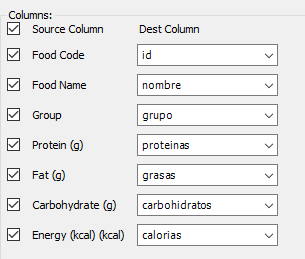
\includegraphics[width=0.4\textwidth]{figures/importacion.png}
    \caption{Importación de los datos usando MySQL Workbench.}
    \label{fig:importacion}
\end{figure}

\subsection{Cambios en la base de datos original}

Para optimizar la base de datos y mejorar el funcionamiento del algoritmo con el fin de alcanzar mejores soluciones, existen ciertos cambios a realizar a los datos aportados por el gobierno de Reino Unido.

El primer cambio es la eliminación de los datos incompletos. En la base de datos original existen diversos alimentos que no presentan toda la información que se va requerir en el trabajo. El principal promotor de este cambio es la existencia de registros que no tienen calorias asignadas (representadas en el archivo Excel con una \textit{''N''}), que han pasado con el valor \textit{0}.

Sin dejar de lado la eliminación de registros, se filtra las categorías de comidas que pueden ser ingeridas por el consumidor. Existen categorías como, por ejemplo, \textit{''Harinas, granos y almidones''} (AA) o \textit{''Grasas y aceites''} (O), que no son consumidas por el usuario como plato único, sino que participan en la cocción o en el acompañamiento del alimento principal. Por lo que se eliminan. También se elimina la categoría \textit{''Bebidas Alcohólicas''} (Q), ya que sería necesario un análisis más exhaustivo y conocer las recomendaciones de los nutricionistas respecto a su consumo. De esta categoría se mantienen la cerveza, el vino, la sidra y el cava, presentes en la dieta mediterránea y de las que la Sociedad Española de Nutrición Comunitaria (SENC) recomienda el consumo opcional, moderado y responsable~\cite{senpiramide}.

También se ha modificado el grupo \textit{''Zumos''} (PE), donde se ha cambiado \textit{PE} por \textit{FE}. Se ha movido al grupo \textit{''Frutas''} (F) porque los zumos son mucho más parecidos a los alimentos de este grupo que al de las bebidas (P).

En el apéndice \ref{ch:grupos-comida} se encuentran todos los grupos con los que se va a trabajar.

Tras los cambios realizados queda un total de 2616 registros. En la figura \ref{fig:ejemplo} se puede ver un ejemplo de algunos de los alimentos.

\begin{figure}[H]
    \centering
    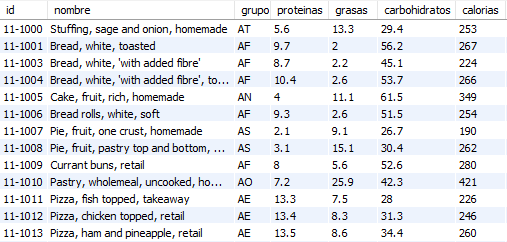
\includegraphics[width=0.65\textwidth]{figures/ejemplo.png}
    \caption{Resultado final de la base de datos.}
    \label{fig:ejemplo}
\end{figure}

\section{Conceptos nutricionales}

Se ha hecho uso de distintas fuentes para los valores nutricionales utilizados para el cálculo de los objetivos, restricciones y límites que se representan en el problema.

En el algoritmo se busca crear un menú equilibrado y personalizado para el usuario, con el propósito de mantener el peso y la masa corporal del individuo.

\subsection{Cálculo de calorías}
\label{ch:calculo-calorias}

El primer objetivo es el calórico, explicado en el apartado \ref{ch:objetivo-restriccion-calorias}. Para ello es necesario saber cuántas kilocalorías diarias necesita el usuario. La Tasa Metabólica Basal (TMB) es la cantidad de energía que el cuerpo necesita para mantener las funciones vitales en reposo. Existen diversas fórmulas de calcularla, pero en este proyecto se hace uso de una las más extendidas actualmente, la fórmula de Harris-Benedict revisada por Mifflin et al.~\cite{mifflin1990}. Esta fórmula toma en cuenta el peso, la altura, la edad y el sexo para estimar las kilocalorías.

\begin{itemize}
    \item Para hombres:
    \[
    \text{TMB} = (10 \times \text{peso en kg}) + (6.25 \times \text{altura en cm}) - (5 \times \text{edad en años}) + 5
    \]
    \item Para mujeres:
    \[
    \text{TMB} = (10 \times \text{peso en kg}) + (6.25 \times \text{altura en cm}) - (5 \times \text{edad en años}) - 161
    \]
\end{itemize}

Como se explica en la definición de la TMB, esta energía es calculada en reposo. Por lo tanto, para alcanzar una aproximación real será necesario multiplicar el resultado por un factor que depende del nivel de actividad física.~\cite{krause2016}

\begin{itemize}
    \item Sedentario (poco o ningún ejercicio): \textit{TMB $\times$ 1.2}
    \item Actividad ligera (ejercicio ligero o deportes 1-3 días a la semana): \textit{TMB $\times$ 1.375}
    \item Actividad moderada (ejercicio moderado o deportes 3-5 días a la semana): \textit{TMB $\times$ 1.55}
    \item Actividad alta (ejercicio intenso o deportes 6-7 días a la semana): \textit{TMB $\times$ 1.725}
    \item Actividad muy alta (ejercicio muy intenso, trabajos físicos o entrenamiento dos veces al día): \textit{TMB $\times$ 1.9}
\end{itemize}

Por ejemplo, para un hombre de \textit{23 años} que pesara \textit{75 kg} y midiera \textit{175 cm} su TMB sería de \textit{1734 kilocalorías por dia}. Pero como también realiza una actividad moderada, habría que multiplicar por \textit{1.55}, dando un total de \textit{2687.31 kcal/dia}.

\begin{comment}
\subsection{Distribución de calorías}

El segundo objetivo es la correcta distribución diaria de calorías. Se busca que los alimentos ingeridos en cada comida (desayuno, tentempié, almuerzo, merienda y cena) estén dentro de unos límites que sean recomendables. Estos límites son, siguiendo las pautas del Ministerio de Sanidad~\cite{alimentacion_saludable}:

\begin{itemize}
    \item $20\% = \% \text{ de kcal en el desayuno}$
    \item $5\% \leq \% \text{ de kcal en el tentempié} \leq 10\%$
    \item $30\% = \% \text{ de kcal en el almuerzo}$
    \item $5\% \leq \% \text{ de kcal en la merienda} \leq 10\%$
    \item $25\% \leq \% \text{ de kcal en la cena} \leq 30\%$
\end{itemize}

Para calcular el porcentaje de nuestras calorías bastaría con sumar los alimentos correspondientes a una comida en particular, dividirlo entre el número de calorías totales consumidas en ese día y multiplicar el resultado por \textit{100}. La fórmula en una comida como el almuerzo es:
\[
\left( \frac{\text{kcal alimento 1} + \text{kcal alimento 2} + \text{kcal bebida}}{\text{kcal totales}} \right) \times 100
\]
\end{comment}

\subsection{Distribución de macronutrientes}
\label{ch:distribucion-macronutrientes}

Otro objetivo, tratado en el punto \ref{ch:objetivo-restriccion-macronutrientes}, es la correcta distribución diaria de macronutrientes, es decir, de los hidratos de carbono, de las proteínas y de las grasas. El \textit{Institute of Medicine (IOM)}, en su trabajo de 2005~\cite{iom2005}, define los AMDR (Acceptable Macronutrient Distribution Ranges) como los rangos de ingesta para macronutrientes que se asocian con un riesgo reducido de enfermedades crónicas y aseguran una ingesta adecuada de nutrientes esenciales. Estos límites para adultos son:

\begin{itemize}
    \item $45\% \leq \% \text{ de carbohidratos} \leq 65\%$
    \item $10\% \leq \% \text{ de proteínas} \leq 35\%$
    \item $20\% \leq \% \text{ de grasas} \leq 35\%$
\end{itemize}

Para saber si la solución respeta estos límites, primero es necesario saber cuántas kilocalorías aporta cada macronutriente. Siguiendo el estudio del \textit{IOM}, las kilocalorías por gramo de cada macronutriente son:

\begin{itemize}
    \item Carbohidratos: \textit{4 kcal} por gramo
    \item Proteínas: \textit{4 kcal} por gramo
    \item Grasas: \textit{9 kcal} por gramo
\end{itemize}

La suma de las kilocalorías individuales de cada macronutriente equivale al total de calorías del alimento, dato del que ya se dispone.

Con las kilocalorías de cada macronutriente ya calculadas, solo falta dividir estas entre las calorías totales y multiplicarlo por \textit{100} para saber los porcentajes de cada macronutriente. Por ejemplo, para calcular el procentaje de carbohidratos sería:
\[
\left( \frac{\text{kcal de carbohidratos}}{\text{kcal totales}} \right) \times 100
\]

Siguiendo el caso de los hidratos de carbono, \textit{11 g} de carbohidratos de un alimento de \textit{98 kcal} representa un porcentaje del \textit{44.9 \%} respecto al total de calorías.


\section{Cromosoma planteado}
\label{ch:solucion-planteada}

Se ha buscado plantear un menú siguiendo los hábitos alimenticios y nutricionales de los consumidores españoles.

La primera parte es la elección de la estructura del cromosoma solución. En este problema se ha planteado que cada gen represente un alimento diferente consumido. Tal y como se muestra en la figura \ref{fig:cromosoma_desarrollo}, cada día del menú semanal consta de un total de 5 comidas repartidas a lo largo del mismo: desayuno, tentempié, almuerzo, merienda y cena. De estas comidas, las tres principales, el desayuno, el almuerzo y la cena, consta cada una de 2 alimentos y 1 bebida, haciendo un total de 3 genes. Las otras dos, el tentempié y la merienda, consideradas como comidas entre horas, tienen 1 alimento cada una, es decir, añadiendo 2 genes más al cromosoma.

Cada día presenta al final 11 genes (o alimentos). Como el proyecto trata de una planificación semanal, se repite esta cadena por cada día de la semana, dando un cromosoma que presenta un total de 77 genes.

\begin{figure}[H]
    \centering
    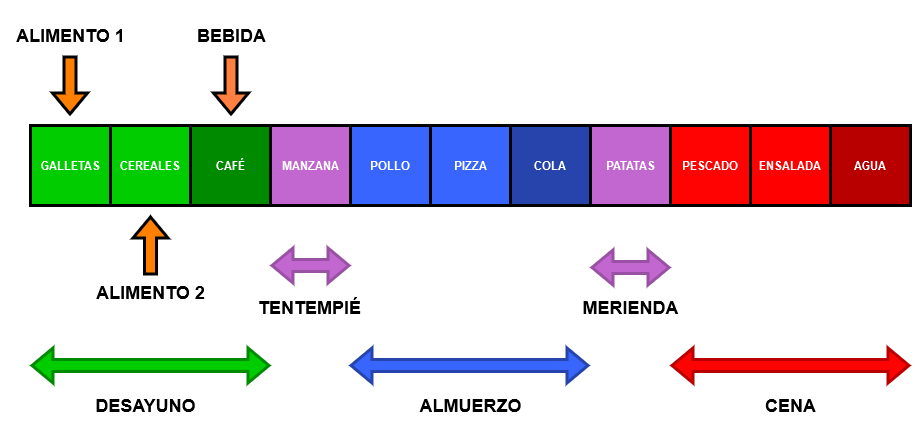
\includegraphics[width=1\textwidth]{figures/cromosoma_desarrollo.png}
    \caption{Estructura de la solución.}
    \label{fig:cromosoma_desarrollo}
\end{figure}

Como se ha explicado, el tercer gen de cada comida principal está reservado para una bebida, por lo que es necesario filtrar los grupos de comida para que seleccione solo un alimento de esta categoría. Estos cambios que se realizan en la inicialización y mutación son explicados en el apartado \ref{ch:explicacion-algoritmo}, pero primero se define qué categorías de alimentos (detalladas en el apéndice \ref{ch:grupos-comida}) están reservadas para ciertos genes o comidas.

\begin{itemize}
    \item El tercer gen de cada comida principal está destinado a una bebida. De las categorías disponibles, solo se puede seleccionar de los grupo \textit{''Bebidas''} (P), \textit{''Jugos de frutas''} (FC), \textit{''Zumos''} (FE) o \textit{''Bebidas Alcohólicas''} (Q) (solo si el sujeto es mayor de edad).
    \item Debido a que la bebida del desayuno suele ser una bebida con leche (no presente en el grupo \textit{P}), café o un zumo, se ha decidido que el valor que tenga este gen sea de las categorías \textit{''Leche de vaca''} (BA), \textit{''Bebidas a base de leche''} (BH), \textit{''Bebidas en polvo, esencias e infusiones''} (PA), \textit{''Jugos de frutas''} (FC) o \textit{''Zumos''} (FE).
    \item También los alimentos del desayuno suelen diferenciarse con respecto a los del almuerzo y la cena, que son comúnmente intercambiables entre sí. Por ello los alimentos de esta comida son del grupo \textit{''Huevos''} (C), \textit{''Frutas''} (FA), \textit{''Bacon''} (MAA) o \textit{''Cereales''} (A), excepto \textit{''Arroz''} (AC), \textit{''Pasta''} (AD) y \textit{''Pizza''} (AE), que se suelen consumir en el almuerzo o la cena.
    \item Para las comidas entre horas, tentempié y merienda, se han seleccionado alimentos de las categorías \textit{''Frutas''} (F) y \textit{''Azúcares''} (S).
    \item Para las otras dos comidas principales, el almuerzo y la cena, los alimentos pueden ser de cualquier grupo, excepto los cereales, salvo \textit{''Panes''} (AF) y las excepciones antes mencionadas: el arroz, la pasta y las pizzas.
\end{itemize}


\section{Objetivos y restricciones}
\label{ch:objetivo-restricciones}
\begin{comment}
Para los objetivos se crean funciones de minimización, donde la solución candidata (o soluciones) con el valor más bajo es la que mayor aptitud presenta.
\end{comment}
\subsection{Objetivo y restricción de calorías}
\label{ch:objetivo-restriccion-calorias}

El primer objetivo que se introduce en el problema es de las kilocalorías. Se busca que la diferencia entre las kilocalorías que el usuario necesita diariamente y la suma de las kilocalorías de todos los alimentos consumidos en un día sea 0 ó lo más cercano posible. La función de evaluación mide cuánto se ha desviado en total en toda la semana, es decir, se va sumando cada desviación de kilocalorías diaria hasta obtener un valor semanal.

Se le pregunta al usuario por distintos atributos físicos y por su nivel de actividad, con lo que se calcula la tasa metabólica basal y, en un última instancia, las kilocalorías, como se explica en el apartado \ref{ch:calculo-calorias}.
\newpage
El objetivo está atado a una restricción \textit{box-constraint}. Se penaliza aquellas desviaciones diarias que superen unos límites superior e inferior del 10\% respecto a las kilocalorías que el usuario necesita. Busca que las soluciones que se alejen bastante del objetivo sean menos seleccionadas.
\begin{small}
\[
    \begin{aligned}
    & \text{Minimizar } f_{\text{calorías}}(c_{i,d}) = \sum_{d=1}^{7} \left| k - \sum_{i=1}^{n_d} c_{i,d} \right| \\
    & \text{Sujeto a } 0.9k \leq \sum_{i=1}^{n_d} c_{i,d} \leq 1.1k, \quad \forall d \in \{1, 2, \ldots, 7\}
    \end{aligned}
    \]

        Donde:
        \begin{itemize}
        \item \( c_{i,d} \) es la cantidad de calorías del alimento \( i \) consumido en el día \( d \).
        \item \( k \) es el objetivo calórico diario.
        \item \( n_d \) es el número total de alimentos consumidos en el día \( d \).
        \end{itemize}
\end{small}


\subsection{Objetivo y restricción de macronutrientes}
\label{ch:objetivo-restriccion-macronutrientes}

Este objetivo trata de distribuir correctamente los macronutrientes a lo largo del día. Se busca que cada tipo de macronutriente se encuentre dentro de los límites recomendado en el apartado \ref{ch:distribucion-macronutrientes}, poniendo como objetivo la media de estos límites. Parecido al anterior objetivo, se calcula la diferencia diaria entre estas medias y los valores reales de proteínas, carbohidratos y grasas obtenidos. Posteriormente, la función evalúa la desviación total en la semana.

Existe también una restricción de caja asociada a este objetivo, donde se requiere que la ingesta diaria de cada macronutriente se encuentre dentro de los límites antes citados.
\begin{small}
    \[
    \begin{aligned}
    & \text{Minimizar } f_{\text{macronutrientes}} = \sum_{d=1}^{7} \Bigg( \left| \frac{\sum_{i=1}^{n_d} C_{i,d}}{\sum_{i=1}^{n_d} E_{i,d}} - 0.55 \right| \\
    & \qquad + \left| \frac{\sum_{i=1}^{n_d} P_{i,d}}{\sum_{i=1}^{n_d} E_{i,d}} - 0.225 \right| + \left| \frac{\sum_{i=1}^{n_d} G_{i,d}}{\sum_{i=1}^{n_d} E_{i,d}} - 0.275 \right| \Bigg) \\
    & \text{Sujeto a } \\
    & \quad 0.45 \leq \frac{\sum_{i=1}^{n_d} C_{i,d}}{\sum_{i=1}^{n_d} E_{i,d}} \leq 0.65, \\
    & \quad 0.10 \leq \frac{\sum_{i=1}^{n_d} P_{i,d}}{\sum_{i=1}^{n_d} E_{i,d}} \leq 0.35, \\
    & \quad 0.20 \leq \frac{\sum_{i=1}^{n_d} G_{i,d}}{\sum_{i=1}^{n_d} E_{i,d}} \leq 0.35, \\
    & \quad \forall d \in \{1, 2, \ldots, 7\}
    \end{aligned}
    \]
\newpage
        Donde:
        \begin{itemize}
        \item \( E_{i,d} \) es la cantidad de energía (calorías) del alimento \( i \) consumido en el día \( d \).
        \item \( C_{i,d} \) es la cantidad de calorías provenientes de carbohidratos del alimento \( i \) consumido en el día \( d \).
        \item \( P_{i,d} \) es la cantidad de calorías provenientes de proteínas del alimento \( i \) consumido en el día \( d \).
        \item \( G_{i,d} \) es la cantidad de calorías provenientes de grasas del alimento \( i \) consumido en el día \( d \).
        \item \( n_d \) es el número total de alimentos consumidos en el día \( d \).
        \end{itemize}
\end{small}

\subsection{Objetivo de preferencia}

Este objetivo busca la personalización del menú incluyendo los grupos de alimentos favoritos del usuario, o exluyendo aquellos que no le gustan. Se favorecerá los grupos preferidos y se penalizará los que no. Se puede considerar como restricción de igualdad débil ya que, aunque penalice las soluciones que la violan, no las invalida. A diferencia de los otros objetivos, esta función de minimización puede alcanzar valores negativos si existe una gran variedad de alimentos con grupo predilecto en la planificación.
\[
\text{Minimizar } f_{\text{preferencia}} = \sum_{i=1}^{N}
\begin{cases} 
-P & \text{si } g(a_i) = G_+ \\
P & \text{si } g(a_i) = G_- \\
0 & \text{en otro caso}
\end{cases}
\]
\begin{small}
    Donde:
    \begin{itemize}
    \item \( f_{\text{preferencia}} \) es la penalización total de preferencia de grupo durante la semana.
    \item \( N \) es el número total de alimentos consumidos en la semana.
    \item \( a_i \) es el alimento \( i \) consumido durante la semana.
    \item \( G_+ \) es el grupo que gusta.
    \item \( G_- \) es el grupo que no gusta.
    \item \( P \) es la penalización de preferencia.
    \item \( g(a_i) \) es el grupo del alimento \( a_i \).
    \end{itemize}
\end{small}

\subsection{Restricción de alergia}

Similar al objetivo de preferencia, es una restricción de igualdad donde se penaliza de gran manera si el usuario es alérgico al grupo del alimento del menú. Al finalizar la semana, se suman todas las penalizaciones de alergias, haciendo que sea inviable para el algoritmo volver a seleccionar un alimento que produzca alergia.
\[
\text{Minimizar } f_{\text{alergia}} = \sum_{i=1}^{N} 
\begin{cases} 
P_{\text{alergia}}^2 & \text{si } g(a_i) = G_{\text{alergia}} \\
0 & \text{en otro caso}
\end{cases}
\]
\begin{small}
    Donde:
    \begin{itemize}
    \item \( f_{\text{alergia}} \) es la penalización total por alergia durante la semana.
    \item \( N \) es el número total de alimentos consumidos en la semana.
    \item \( a_i \) es el alimento \( i \) consumido durante la semana.
    \item \( G_{\text{alergia}} \) es el grupo al que el usuario es alérgico.
    \item \( P_{\text{alergia}} \) es la penalización fuerte por alergia.
    \item \( g(a_i) \) es el grupo del alimento \( a_i \).
    \end{itemize}
\end{small}

\section{Construcción del algoritmo}
\label{ch:explicacion-algoritmo}

El código completo se encuentra en el repositorio de Github del autor~\cite{quesada_nutritionplanning}.

La biblioteca usada para la creación del algoritmo evolutivo ha sido \textit{Pymoo}. \textit{Pymoo} es un framework de \textit{Python} diseñado para la optimización multiobjetivo. Entre sus ventajas se encuentran la amplia gama de algoritmos para abordar los problemas, como \textit{NSGA-II}, \textit{SPEA2} o \textit{MOEA/D}. Permite modificar fácilmente los operadores de selección, cruce y matación, lo que ayuda a la personalización del algoritmo según el problema. Además, \textit{Pymoo} presenta un conjunto de herramientas de visualización para la interpetación de resultados, permitiendo entender el comportamiento de los algoritmos.~\cite{pymoo}

Se ha creado una clase personalizada que hereda de \textit{''ElementwiseProblem''}, ya que esta última proporciona una estructura eficiente para evaluar cada solución individualmente, como se muestra en el listado \ref{lst:planning}.
\newpage
\begin{lstlisting}[basicstyle=\ttfamily, caption=Clase para la evaluación.,label={lst:planning}]
    CLASE PlanningComida extiende ElementwiseProblem
    
        MÉTODO __init__(self, num_variables, limites_variables,
                            num_objetivos, num_restricciones)
            INICIALIZAR num_variables
            INICIALIZAR limites_variables
            INICIALIZAR num_objetivos
            INICIALIZAR num_restricciones
            LLAMAR al constructor de ElementwiseProblem
    
        MÉTODO evaluate(self, solución, out)
            CALCULAR valores_objetivo
            CALCULAR valores_restricciones
            out["F"] = valores_objetivo
            out["G"] = valores_restricciones
\end{lstlisting}

El primer método creado es \textit{''\_\_init\_\_''}, que inicializa los parámetros del problema, incluyendo el tamaño de la solución (77 genes), el número de objetivos y restricciones (3 cada uno) y los límites del problema (el tamaño de la base de datos).

El segundo método es \textit{''evaluate''}, que es donde se define cómo se evalúan las soluciones. Este método recibe una solución individual y calcula su aptitud a partir de los objetivos y restricciones definidos en el apartado \ref{ch:objetivo-restricciones}.

Se recorre la cadena y, por cada gen, se extraen las calorías, el grupo y los macronutrientes. Se comprueba el objetivo de la preferencia comparando el grupo del alimento con los grupos de preferencia del usuario y, en caso de ser necesario, se suma una penalización a una variable que contará todas las sanciones totales de la solución respecto a este objetivo. El mismo procedimiento se hace con la restricción de la alergia.

Por cada 11 genes de la cadena (que representa un día) se comprueba el objetivo calórico, donde la desviación de kilocalorías diarias respecto al objetivo marcado para el usuario se suma a un contador que refleja la desviación semanal total. Este es el valor a minimizar. Pero, además, existe otro contador que suma todas las penalizaciones de la restricción calórica. Cada vez que las kilocalorías diarias se sale de los límites del 10\% se agrega una penalización a este contador. Este es otro valor que se busca minimizar.

El cálculo de los valores a minimizar del objetivo y restricción de macronutrientes sigue el mismo proceso que el de las calorías.

Los resultados de las evaluaciones se almacenan en los diccionarios \textit{''out[F]''} y \textit{''out[G]''}. \textit{''out[F]''} contiene los valores de las funciones objetivos, que intentamos optimizar. \textit{''out[G]''}, muy usado en métodos separatistas para el manejo de restricciones, contiene los valores de las restricciones que deben ser satisfechas para que las soluciones se consideren factibles. Si se usase, por ejemplo, métodos de penalización para las restricciones, no sería necesario incluir \textit{''out[G]''}, ya que las restricciones se tratan como funciones objetivo. 

Tras la creación de la clase, hay que crear una función que recoja los resultados de esta clase para incluirlos en el algoritmo evolutivo. El funcionamiento del algoritmo es, en esencia, el mismo que se ha explicado en la sección \ref{ch:marco-teorico}, aunque se puede modificar o añadir algún operador según el tipo de algoritmo usado, razón de la experimentación con distintos algoritmos del apartado \ref{ch:algoritmos-multiobjetivo}. Por lo tanto, lo primero a seleccionar es el algortimo con el que se va a trabajar, ya sea NSGA-II, MOEA/D, etc.

Se selecciona el número de individuos por generación y el número de generaciones que el algoritmo evaluará. Como no se ha puesto ninguna condición de parada específica el algoritmo terminará tras haber evaluado todas las generaciones predefinidas.

Lo primero que el algoritmo hace es crear la matriz en la que se aloja toda la población, que tiene un tamaño del número de genes (o variables) por solución multiplicado por el número de individuos de una generación. Por ejemplo, si el menú se compone de \textit{77} genes y se selecciona un tamaño de población de \textit{100} indiviudos, se crea una matriz de \(100 \, individuos \times 77 \, genes\), en la que cada solución candidata se evalúa individualmente.

\textit{Pymoo} dispone de varios métodos de incialización, entre los que destaca \textit{''IntegerRandomSampling''}, usado para la generación de matrices de enteros. Este se puede usar en el planificador de comidas al seleccionar el índice del alimento que se añade al menú, el cual es un número entero. Pero se ha decidido crear una versión modificada del mismo para que genere soluciones que sean interesantes en el contexto del proyecto. En vez de seleccionar un índice aleatorio de un alimento de la base de datos, selecciona basándose en las características propias de la solución, explicadas en el apartado \ref{ch:solucion-planteada}. Es decir, se ha configurado para que se seleccione una bebida cuando el gen sea el tercero de una comida principal o para que los alimentos del desayuno sean de la categoría \textit{''Cereales''} (A), por ejemplo. Así se consigue que la primera población de la generación cumpla las particularidades del problema, como se observa en la figura \ref{fig:matriz-inicializacion}.

\begin{figure}[H]
    \centering
    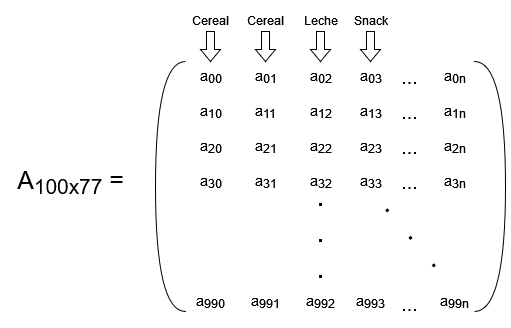
\includegraphics[width=0.75\textwidth]{figures/matriz-inicializacion.png}
    \caption{Matriz de inicialización.}
    \label{fig:matriz-inicializacion}
\end{figure}

Cada solución de esta población es evaluada según lo explicado al comienzo de este apartado. Si no ha llegado al número total de generaciones, el algoritmo se prepara para generar una nueva población a partir de los operadores.

En la selección se eligen individuos de la población basado en la aptitud. En este caso concreto los valores más bajos presentarán una mayor aptitud, al ser funciones de minimización. Se va a usar la selección por torneo, predeterminada por \textit{Pymoo} para este tipo de problemas.

Tras elegir los individuos, se cruzan para la generación de una nueva población.  Se puede variar entre el cruce de un punto y el de dos puntos, asignándoles a cada uno de ellos una probabilidad de cruce \(P_c\)  . Aparte de los mecanismos elitistas que usen los algoritmos multi-objetivo, no se ha realizado ningún método extra de selección ambiental, por lo que se realiza un reemplazo generacional completo.

Para la mutación ocurre como con la inicialización. En vez de elegir un método de los que ofrece \textit{Pymoo}, se ha decido crear un método personalizado. El nuevo método recorre cada individuo creado en el cruce y decide si el gen es reservado para una bebida, para un snack, etc. Con una probabilidad \(P_m\) a determinar, muta una bebida por otra bebida o un alimento de una categoría determinada por otro de la misma categoría, como se muestra en la figura \ref{fig:mutacion-custom}. Esto logra, junto con la inicialización, que todas las soluciones a lo largo de las generaciones cumplan con las peculiaridades de este problema.

\begin{figure}[H]
    \centering
    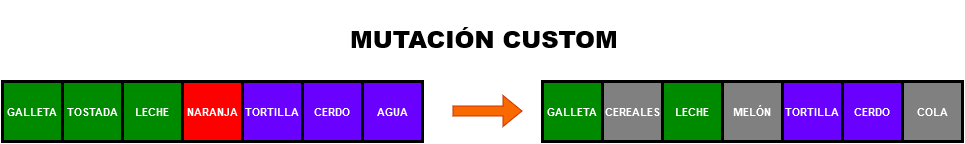
\includegraphics[width=1\textwidth]{figures/mutacion-custom.png}
    \caption{Mutación personalizada.}
    \label{fig:mutacion-custom}
\end{figure}

Por último, esta nueva población resultante vuelve a ser evaluada en busca de ser óptima para el problema.

El algortimo evolutivo se ejecuta utilizando la función \textit{''minimize''} de \textit{Pymoo}, que toma el problema y la configuración del algoritmo. Como se muestra en la tabla \ref{tab:optimizacion}, el algoritmo va avanzando en busca de mejores soluciones.

En la tabla se aprecia, en orden: \textit{''n\_gen''} muestra el número de generación, \textit{''n\_eval''} es el contador de evaluaciones de individuos, \textit{''n\_nds''} es el número de soluciones no dominadas encontradas, \textit{''cv\_min''} es el valor mínimo de violación de una población, \textit{''n\_avg''} es el valor promedio de violación de una población, \textit{''eps''} es una métrica que mide la convergencia del algoritmo hacia soluciones óptimas e \textit{''indicator''} se usa para clasificar la calidad del frente de Pareto en cada generación.

\begin{table}[h!]
    \centering
    \small % Reduce el tamaño del texto
    \begin{tabularx}{\textwidth}{@{}ccccccc@{}}
        \toprule
        \textbf{n\_gen} & \textbf{n\_eval} & \textbf{n\_nds} & \textbf{cv\_min} & \textbf{cv\_avg} & \textbf{eps} & \textbf{indicator} \\ 
        \midrule
         1 &   100 &  1 & 2.415619E+03 & 5.717019E+03 &          - &          - \\ 
         2 &   200 &  1 & 1.789955E+03 & 4.574975E+03 &          - &          - \\ 
         3 &   300 &  1 & 1.290943E+03 & 3.787494E+03 &          - &          - \\ 
         4 &   400 &  1 & 1.195388E+03 & 3.107680E+03 &          - &          - \\ 
         5 &   500 &  1 & 1.070258E+03 & 2.478680E+03 &          - &          - \\ 
         6 &   600 &  1 & 0.000000E+00 & 1.867363E+03 & 1.0000000000 &     ideal \\ 
         7 &   700 &  2 & 0.000000E+00 & 1.400831E+03 & 0.5000000000 &     ideal \\ 
         8 &   800 &  3 & 0.000000E+00 & 9.870077E+02 & 0.2500000000 &         f \\ 
         9 &   900 &  4 & 0.000000E+00 & 6.756844E+02 & 0.1250000000 &     ideal \\ 
        10 &  1000 &  5 & 0.000000E+00 & 4.510310E+02 & 0.0625000000 &     ideal \\ 
        \bottomrule
    \end{tabularx}
    \caption{Resultados del algoritmo genético.}
    \label{tab:optimizacion}
\end{table}

El algortimo, con este manejo de restricciones, está configurado para que, hasta que no alcance una solución viable (\textit{''cv\_min''}=0), no empieza a evaluar la convergencia y la calidad del frente de Pareto.

En el caso de que, como se ha explicado antes, no fuera necesario \textit{''out[G]''} por el manejo de las restricciones, simplemente desaparecen \textit{''cv\_min''} y \textit{''cv\_avg''}, y \textit{''n\_nds''}, \textit{''eps''} e \textit{''indicator''} se calculan desde la primera generación.

Todas las métricas que obtiene el algoritmo son guardadas en una variable \textit{''resultado''}, a la que se puede acceder.

\begin{itemize}
    \item En \textit{''resultado.X''} se encuentra una matriz que contiene las soluciones no dominadas encontradas. En este proyecto son cada uno de los posibles menús factibles que el algoritmo ha encontrado. Siguiendo el ejemplo \ref{tab:optimizacion}, en 10 generaciones el algoritmo ha encontrado 5 soluciones no dominadas, por lo que la matriz tiene un tamaño de \(5 \, n\_nds\ \times 77 \, genes\).
    \item En \textit{''resultado.F''} se encuentra una matriz que contiene los valores de las funciones objetivo para cada solución no dominada encontrada. Como el algoritmo presenta 3 objetivos, la matriz puede tener un tamaño de \(5 \, n\_nds \times 3 \, objetivos\).
    \item En \textit{''resultado.G''} se encuentra una matriz muy parecida a \textit{''resultado.F''}, pero con las restricciones en vez de los objetivos. Esta matriz se encuentra vacía si los objetivos y las restricciones no se tratan de manera separada.
\end{itemize}

\subsection{Manejo de restricciones}
\label{ch:manejo-restricciones}

\subsubsection{Penalización estática}
\label{ch:penalizacion-estatica}

En este método se penalizan las soluciones que violan las restricciones. En las funciones en las que se definen las restricciones de calorías y macronutrientes, se calcula una penalización proporcional a la diferencia entre el objetivo y los nutrientes consumidos, multiplicada por una constante de penalización, mostradas en el listado \ref{lst:factores}. Poniendo de ejemplo la restricción de calorías, si el objetivo calórico es 2500 kilocalorías y la diferencia con las kilocalorías ingeridas está fuera del 10\%, se multiplica esa diferencia por un factor de penalización. Por lo tanto, cuanto mayor es la diferencia, mayor es la penalización, lo que ayuda a guiar al algoritmo en busca de soluciones que se penalicen menos y, en última instancia, que se acerquen lo máximo posible al objetivo.

En el caso de la restricción de alergia, se penaliza con un factor de penalización si el grupo alérgico aparece en el menú. Si no aparece, se devuelve 0. Tras realizar diversos tests, se ha llegado a la conclusión de que el algoritmo encuentra mejores resultados si el factor de penalización se eleva al cuadrado, lo que hará inviable buscar soluciones que incumplan esta restricción.
\newpage
En el objetivo de preferencias, que se puede considerar una restricción débil, se penaliza con un factor de penalización (de menor valor que el de la alergia) en el caso de que aparezca en el menú un grupo de alimentos que disguste al usuario. En cambio, si el alimento es del gusto del individuo, se devuelve ese mismo factor con un signo negativo delante, lo que ayuda a que baje el valor a minimizar.

Los valores retornados de las funciones de restricción se suman entre sí. El valor resultante se suma a cada uno de los valores objetivo del problema. El algoritmo pasa de calcular 3 objetivos y 3 restricciones a calcular solo los 3 objetivos a los que se le ha sumado la penalización de las restricciones.

\begin{lstlisting}[basicstyle=\ttfamily, caption=Factores de penalización.,label={lst:factores}]
    PENALIZACION_CALORIAS = 50
    PENALIZACION_MACRONUTRIENTES = 30
    PENALIZACION_PREFERENCIA = 10
    PENALIZACION_ALERGIA = 100
\end{lstlisting}

\subsubsection{Método separatista}
\label{ch:metodo-separatista}

En el método separatista los objetivos y las restricciones se tratan por separado. A diferencia de los métodos de penalización, en las funciones de restricción no se hace uso de los factores. Se devuelve únicamente, en el caso de las restricciones de las calorías y los macronutrientes, la diferencia entre el valor objetivo y el valor obtenido de la solución candidata.

La función de la restricción de la alergia (y la de las preferencias) se trata igual que en los métodos con penalización, por lo que aquí sí que se usa el factor de penalización correspondiente.

En \textit{''out[F]''} se introducen los valores de las funciones de los objetivos (3 en total), y en \textit{''out[G]''} se introducen los valores de las funciones de las restricciones (3). El algoritmo busca primero soluciones que no violen las restricciones y, cuando las encuentra, busca soluciones que optimicen el problema. En la tabla \ref{tab:optimizacion} se puede ver este funcionamiento.

\subsubsection{Restricciones como objetivo}
\label{ch:restricciones-objetivo}

Si bien en los anteriores casos se desarrollaron versiones personalizadas de los métodos, en este tercer caso se va a hacer uso de la herramienta de \textit{Pymoo} \textit{''ConstraintsAsObjective''}~\cite{pymoo_constraints_as_obj}.

Este método se caracteriza por incorporar las restricciones como objetivos. La finalidad no es solo encontrar soluciones que cumplan con todas las restricciones, sino también evaluar cuánto se puede mejorar la optimización si se relajan las restricciones. La construcción del método de evaluación se realiza igual que en el método separatista. El cambio se lleva a cabo en la función de optimización, donde se indica que en el algoritmo a minimizar se empleará \textit{''ConstraintsAsObjective''}.
\section{Interfaz gráfica}
\label{ch:interfaz-grafica}

Si bien el objetivo principal de este PFG es la construcción del algoritmo evolutivo y la experimentación del mismo (apartado \ref{ch:objetivos}), se ha creado una interfaz simple que sirve de guía para la ejecución del algoritmo. Se ha hecho uso de la biblioteca \textit{''tkinter''} para ello~\cite{python_tkinter}.

La ventana principal, que es la que se muestra en la figura \ref{fig:ventana-main}, es el punto de entrada para la ejecución del algoritmo. Se ha nombrado \textit{''Planificación nutricional mediante algoritmos evolutivos''}. Dispone de un título, que comparte con el nombre de la ventana, y dos botones. El botón de la izquierda, \textit{''Planificar el menú''}, lleva a la ventana que se encuentra en la figura \ref{fig:ventana-usuario}, que es donde se le pregunta al usuario para poder calcular sus kilocalorías necesarias y sus preferencias alimenticias. El segundo botón, \textit{''Visualizar la base de datos''}, redirige a la ventana \textit{''Base de datos''}, mostrada en la figura \ref{fig:ventana-basedatos}. Aquí se indica cada alimento con sus grupo y sus valores nutricionales.

\begin{figure}[H]
    \centering
    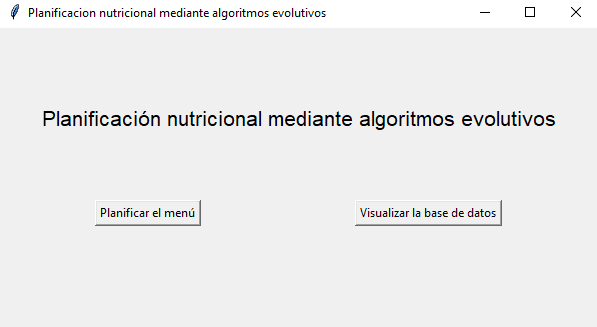
\includegraphics[width=0.9\textwidth]{figures/ventana-main.png}
    \caption{Ventana principal.}
    \label{fig:ventana-main}
\end{figure}

En la ventana \textit{''Base de datos''}, figura \ref{fig:ventana-basedatos}, se ha creado un \textit{''TreeView''} para la representación de los datos. Es una herramienta que permite visualizar y gestionar datos en una estructura de árbol. En este caso tiene una forma de tabla y muestra una lista completa de alimentos, cada uno con su categoría, sus calorías y sus macronutrientes. Además, asociado a este \textit{''TreeView''}, se ha creado un \textit{scrollbar} vertical para poder navegar entre los numerosos alimentos.

Se ha incluido un botón \textit{''Volver''} que redirige a la ventana principal \textit{''Planificación nutricional mediante algoritmos evolutivos''}.

\begin{figure}[H]
    \centering
    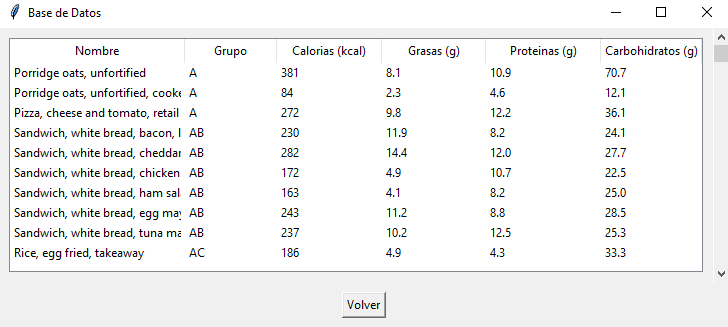
\includegraphics[width=0.9\textwidth]{figures/ventana-basedatos.png}
    \caption{Ventana de la base de datos.}
    \label{fig:ventana-basedatos}
\end{figure}

La ventana \textit{''Preguntas al usuario''}, figura \ref{fig:ventana-usuario}, es usada para calcular las kilocalorías que el usuario necesita y sus grupos alimenticios de preferencia.

Se pregunta al usuario por medio de un \textit{''label''} y este responde en un \textit{''entry''}, que almacena la respuesta. Así ocurre con las preguntas sobre el peso, la edad y la altura. Para el sexo y el nivel de actividad se ha hecho uso de un \textit{''combobox''}, que permite introducir varias opciones posibles dentro de una lista. Para la alergia y las preferencias alimenticias se ha utilizado \textit{''listbox''}, que permite mostrar, bien tabulados, todos los grupos de alimentos. Se puede hacer selección múltiple. Estos grupos quedan guardados para luego usarlos durante la ejecución del algoritmo.

El botón \textit{''Calcular calorías''} activa el cálculo de las kilocalorías objetivo del usuario y las muestra. El botón \textit{''Mostrar menú''} activa la ejecución del algoritmo para que encuentre una solución óptima. El último botón, \textit{''Volver''}, regresa a la ventana principal.

\begin{figure}[H]
    \centering
    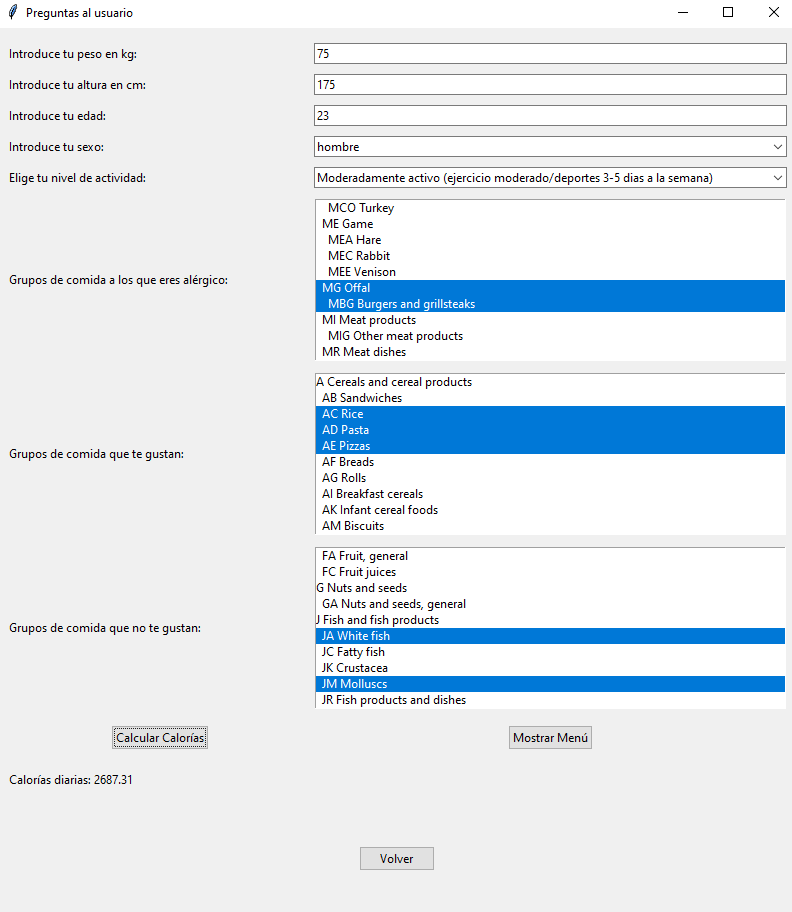
\includegraphics[width=1\textwidth]{figures/ventana-preguntasusuario.png}
    \caption{Ventana de las preguntas al usuario.}
    \label{fig:ventana-usuario}
\end{figure}
\newpage
Tras pulsar el botón \textit{''Mostrar menú''}, el algoritmo se ejecuta con los datos introducidos. Cuando termina, se selecciona la primera de las soluciones no dominadas y se obtiene un menú compuesto por 77 alimentos.

Se ha creado la ventana \textit{''Menú Generado''}, mostrada en la figura \ref{fig:ventana-menu}, donde se ha hecho uso de un \textit{''grid''}, muy útil para la creación de tablas estáticas. Se han introducido 5 filas (comidas diarias) por 7 columnas (días de la semana). Se muestran todos los alimentos que componen la solución elegida, además del grupo al que pertenecen. Se han añadido una fila y una columna como cabeceras, correspondientes a las comidas del día y a los días de la semana, respectivamente. Además, se ha incorporado una fila al final para ayudar a entender si la solución escogida cumple con los objetivos de las kilocalorías y los macronutrientes.

Se han añadido dos botones, \textit{'Atrás''} y \textit{'Cerrar''}. El primero vuelve a la ventana \textit{''Preguntas al usuario''} para la posibilidad de generar otro menú distinto. El segundo botón termina con la ejecución del programa.

\begin{figure}[H]
    \centering
    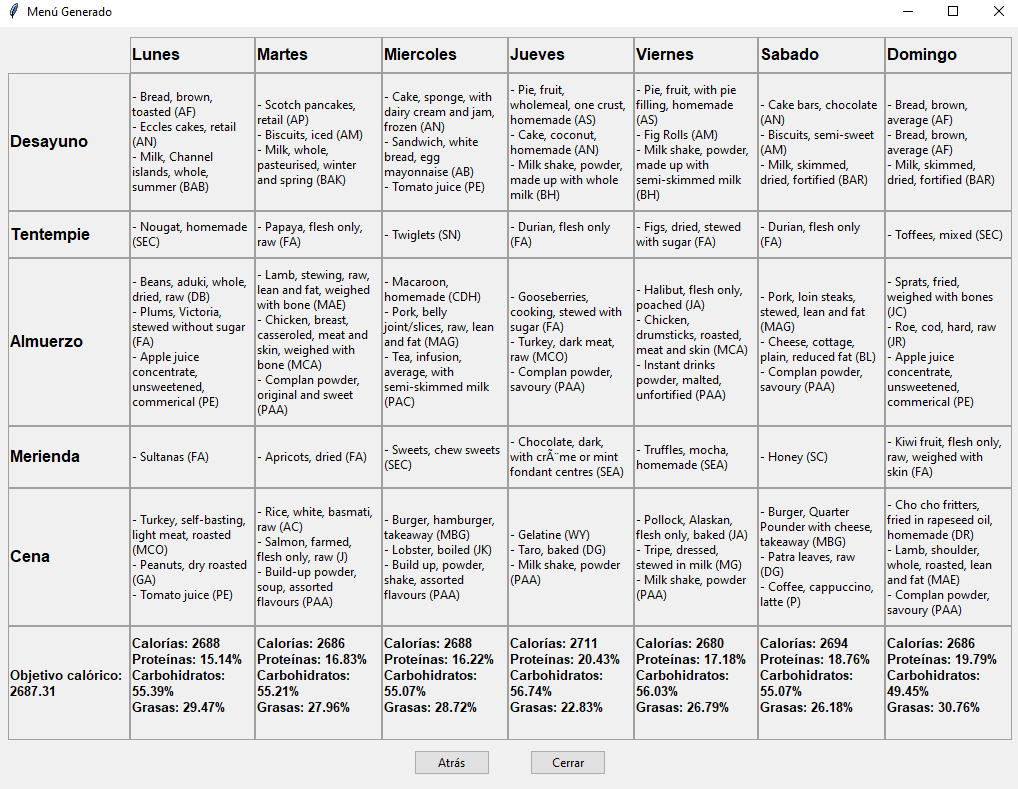
\includegraphics[width=0.965\textwidth]{figures/ventana-menu.png}
    \caption{Ventana del menú generado.}
    \label{fig:ventana-menu}
\end{figure}